\documentclass[leqno]{beamer}
\usepackage{setspace,graphicx,hyperref}
\usepackage{amsfonts,amsthm,amsmath}
\usepackage{caption}
\usepackage{xcolor}
\definecolor{Vandygold}{RGB}{207, 174, 112}
\definecolor{Vandyoak}{RGB}{148, 110, 36}
%% \definecolor{Vandywarmsand}{RGB}{190, 173, 154}
\definecolor{academicdarkblue}{RGB}{40, 45, 78}
%% \definecolor{academicmediumblue}{RGB}{0, 93, 131}
\definecolor{academiclightblue}{RGB}{0, 131, 169}
\usepackage{multicol}
\usepackage{textpos}
\usepackage{tikz}
\usepackage[authoryear]{natbib}
\usepackage[linesnumbered,algoruled,boxed,lined]{algorithm2e}
\usepackage{algorithmic}
\hypersetup{
	colorlinks=true,
	citecolor=blue,
	linkcolor=academicdarkblue
}
\usepackage{multirow}
\usepackage{booktabs}
\usepackage{bm}
\usepackage[default]{opensans}
\usepackage[T1]{fontenc}

\usetheme{Madrid}
\usecolortheme[named=Vandygold]{structure}
\usebackgroundtemplate{
	
\includegraphics[height=\paperheight,
	width=\paperwidth]{VUMC_Background.png};
}

%% \setbeamercovered{transparent}
\setbeamertemplate{itemize item}[circle]
\setbeamertemplate{enumerate item}[default]
\setbeamertemplate{section in toc}[default]
\setbeamerfont{section in toc}{series=\bfseries}
\setbeamercolor{section in toc}{fg=academiclightblue}
\setbeamertemplate{subsection in toc}[default]
\setbeamertemplate{caption}[numbered]
\setbeamerfont{caption name}{series=\bfseries}
\setbeamercolor{caption name}{fg=Vandyoak}

% comments
\newcommand{\blue}[1]{\textcolor{blue}{#1}}
\newcommand{\red}[1]{\textcolor{red}{#1}}

% notations

% consistent with R manual
\newcommand{\pkg}[1]{{\normalfont\fontseries{b}\selectfont #1}}
\let\proglang=\textsf 
\let\code=\texttt

% relative path (graphics)
\graphicspath{{./}, {../figures/}}

\AtBeginSection[]{
	{\setbeamertemplate{background}{
			
\includegraphics[height=\paperheight,
			width=\paperwidth]{VUMC_Background_Sec.jpg};
			\begin{tikzpicture}[overlay, remember picture]
				\node[xshift=-1.75cm,yshift=1cm] at (current 
				page.south east){
					
\includegraphics[width=3cm]{VUMC_Logo_White.png}
				};
			\end{tikzpicture}
		}
		\begin{frame}[plain]
			\begin{NoHyper}
				\centering
				\bfseries
				\setbeamercolor{normal text}{fg=white}
				\usebeamercolor[fg]{normal text}
				\usebeamerfont{title}\insertsectionhead\par%
			\end{NoHyper}
		\end{frame}
	}
}

\renewcommand*{\bibfont}{\scriptsize}

\title[Short Title]{Full Title}
\subtitle[Short Subtitle]{Full Subtitle}
\author[Author Name]{{\sc Author Name}}
\institute[Institution]{Department Name \\ Institution Name}
\date[Date]{Event Name \\ Presentation Date}


\logo{
	\begin{tikzpicture}[overlay, remember picture]
		\node[xshift=-1.75cm,yshift=1cm] at (current page.south east)
		{
\includegraphics[width=3cm]{VUMC_Logo.png}
		};
	\end{tikzpicture}
}

\begin{document}
	
	\begin{frame}[plain]
		\titlepage
	\end{frame}
	
	\begin{frame}
		\frametitle{Overview}
		\begin{NoHyper}
			\tableofcontents
		\end{NoHyper}
	\end{frame}
	
	\section{Section 1}
	
	\begin{frame}
		\frametitle{Add Bullet Points}
		\begin{itemize}
			%%\setlength\itemsep{1em}
			\item My first statement
			\item My second statement
			\item My third statement
		\end{itemize}
	\end{frame}
	
	\begin{frame}
		\frametitle{Add References}
		\begin{itemize}
			%%\setlength\itemsep{1em}
			\item My first reference~\citep{ref1}
			\item My second reference~\citep{ref2}
			\item My third reference~\citep[][Chapter 1]{ref3}
		\end{itemize}
	\end{frame}
	
	\section{Section 2}
	
	\begin{frame}
		\frametitle{Add Formulae}
		My first formula:
		\[Y_{i} = \beta_0 + \beta_1 X_i + \varepsilon_i.\]
		My second formula:
		\begin{align}
			Y_{ij} &= \beta_0 + \beta_1 X_{ij} + b_{i} + 
			\varepsilon_{ij}, \label{eq:myeq1}
			\\ b_i &= b + u_i. \label{eq:myeq2}
		\end{align}
		My third formula:
		\[
		X = 
		\begin{cases}
			1, &\text{w.p. } p;
			\\0, &\text{w.p. } 1 - p.
		\end{cases} 	
		\]
	\end{frame}
	
	\begin{frame}[fragile]
		\frametitle{Add An Algorithm}
		\begin{algorithm}[H]
			\begin{algorithmic}[1]
				\FOR{$i = 1$ to $n$}
				\FOR{$j = 1$ to $m$}
				\STATE $\text{logit}(p_{ij}) = \beta_0 + X_{ij}$
				\STATE $A_{ij} \sim \text{Bernoulli}(p_{ij})$
				\ENDFOR
				\ENDFOR
			\end{algorithmic}
			\caption{My algorithm caption}
			\label{alg:myalg}
		\end{algorithm}
	\end{frame}
	\section{Section 3}
	
	\begin{frame}
		\frametitle{Add A Table}
		\begin{table}[tbp]
			\centering
			\setlength{\tabcolsep}{3.7pt}
			\footnotesize
			\begin{tabular}{c ccc ccc ccc}
				\toprule
				& \multicolumn{3}{c}{Case 1}
				& \multicolumn{3}{c}{Case 2}
				& \multicolumn{3}{c}{Case 3}
				\\
				\cmidrule(lr){2-4} \cmidrule(lr){5-7} 
				\cmidrule(lr){8-10}
				& Type 1 & Type 2 & Type 3 & Type 1 & Type 2 & Type 
				3 & 
				Type 1 & Type 2 & Type 3 \\
				\midrule
				Var 1 & 1.00 & 1.00 & 1.00 & 1.00 & 1.00 & 1.00 
				& 1.00 & 1.00 & 1.00 \\ 
				Var 2 & 1.00 & 1.00 & 1.00 & 1.00 & 1.00 & 1.00 
				& 1.00 & 1.00 & 1.00 \\ 
				Var 3 &1.00 & 1.00 & 1.00 & 1.00 & 1.00 & 1.00 
				& 1.00 & 1.00 & 1.00 \\ 
				\bottomrule
			\end{tabular}
			\caption{My table caption}
			\label{tab:mytab}
		\end{table}
	\end{frame}
	
	\begin{frame}
		\frametitle{Add A Figure}
			\begin{figure}
				\centering
				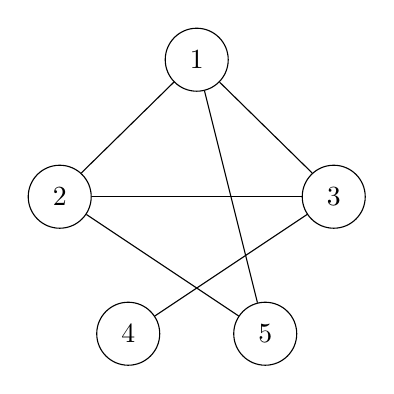
\begin{tikzpicture}[scale=0.87]
					\draw (0, 4) node[draw=black, circle, minimum 
					size=0.8cm] (v1) {$1$};
					\draw (-2, 2) node[draw=black, circle, minimum 
					size=0.8cm] (v2) {$2$};
					\draw (2, 2) node[draw=black, circle, minimum 
					size=0.8cm] (v3) {$3$};
					\draw (-1, 0) node[draw=black, circle, minimum 
					size=0.8cm] (v4) {$4$};
					\draw (1, 0) node[draw=black, circle, minimum 
					size=0.8cm] (v5) {$5$};
					\draw (v1) -- (v2);
					\draw (v1) -- (v3);
					\draw (v1) -- (v5);
					\draw (v2) -- (v3);
					\draw (v2) -- (v5);
					\draw (v3) -- (v4);
				\end{tikzpicture}
				\caption{My figure caption}
				\label{fig:myfig}
			\end{figure}
	\end{frame}
	
	\begin{frame}
		\frametitle{Links and Hyperlinks}
		\begin{itemize}
			\item Go to Algorithm~\ref{alg:myalg}
			\item Go to Table~\ref{tab:mytab}
			\item Go to Figure~\ref{fig:myfig}
			\item Go to Equation~\eqref{eq:myeq1}
			\item Go to \url{https://www.vumc.org/main/home}
			\item Go to \href{https://www.vumc.org/main/home}{this 
			website}
			\item Email to 
			\href{mailto:john.dow@company.com}{john.dow@company.com}
		\end{itemize}
	\end{frame}
	
	\begin{frame}[allowframebreaks]
		\frametitle{References}
		\nocite{*}
		\bibliographystyle{chicago}
		\bibliography{ref}
	\end{frame}
	
	{\usebackgroundtemplate{
			
\includegraphics[height=\paperheight, 
			width=\paperwidth]{VUMC_Background_Sec.jpg}
			\begin{tikzpicture}[overlay, remember picture]
				\node[yshift=2.3cm] at (current 
				page.south){
					
\includegraphics[width = 
					0.5\paperwidth]{VUMC_Logo_White.png}
				};
			\end{tikzpicture}}
		\begin{frame}[plain]
			\begin{center}
			{\huge \bfseries \textcolor{white}{Thank You!}}
		\end{center}
		\end{frame}
	}

\end{document}